Der erste Prototyp soll es ermöglichen, Kratzer und ähnliche Defekte auf transparenten Objekten mittels der Deflektometrie sichtbar zu machen.
Der Ansatz zur Erkennung basiert auf der Idee aus Abbildung \ref{img:scratch}.
Dabei nutzt man die abweichende Lichtreflexion an Kratzern und Defekten im Vergleich zur idealen spiegelnden Oberfläche des Objekts.

\begin{figure}[H]
	\centering
	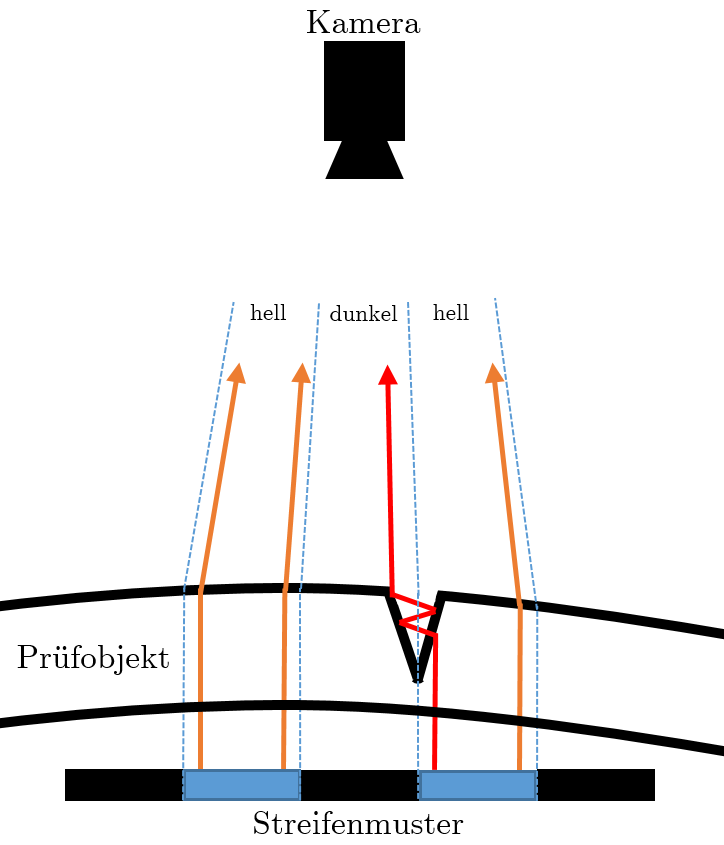
\includegraphics[width=0.5\textwidth]{03_sichtpruefungDurchLichtreflexionen/verfahren/figures/scratch_reflection}
	\caption[Lichtbrechung an einem Kratzer]{Lichtbrechung an einem Kratzer (Abbildung nicht maßstabsgetreu)}
	\label{img:lightreflection}
\end{figure}

\noindent
In Abbildung \ref{img:lightreflection} wird schematisch die Überlegung hinter dem Ansatz dargestellt.
Man nimmt ein Streifenmuster und projiziert dieses auf ein spiegelndes Prüfobjekt.
Für ein transparentes Prüfobjekt kann man das Streifenmuster als Durchlichtbeleuchtung von unten projizieren.
An den Hell-Dunkelübergän\-gen fällt Licht vom hellen Streifen in den Kratzer.
Durch den Kratzer werden manche Lichtstrahlen so reflektiert, dass diese an der Stelle des dunklen Streifens in die Kamera gelangen.
Dadurch erkennt man im Kamerabild eine lokale Fehlstelle, da der Kratzer heller ist als der umliegende dunkle Streifen.
Analog dazu erkennt man im hellen Streifen lokal eine etwas dunklere Stelle.
Durch Anpassung der Kameraeinstellungen kann man beeinflussen, wie stark man den Kratzer sieht.
Z. B. kann dies durch die Erhöhung der Belichtungszeit oder weitere Öffnung der Blende geschehen.
Dadurch wird ein Oberflächendefekt im dunklen Streifen zwar besser und stärker sichtbar, allerdings verliert man die Informationen über den Defekt im hellen Streifen.
Dies liegt daran, dass auch die dunklere Stelle im hellen Streifen so hell werden kann, dass sie nicht mehr von dem hellen Streifen selbst zu unterscheiden ist.
Dieses Problem erkennt man in der Abbildung \ref{img:scratches}.

\begin{figure}[H]
	\centering
	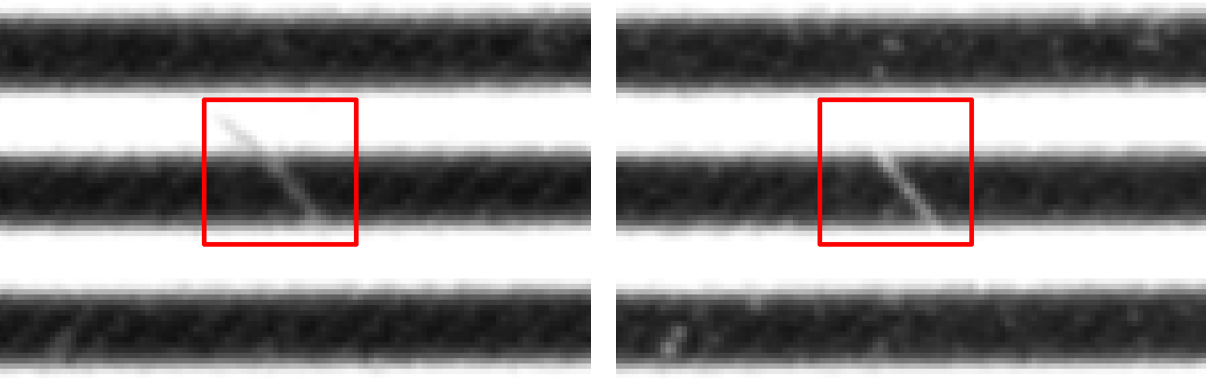
\includegraphics[width=\textwidth]{03_sichtpruefungDurchLichtreflexionen/verfahren/figures/visibleScratch}
	\caption[Kratzer]{Kratzer an Hell-Dunkel-Übergang. Links mit weniger weit geöffneten Blende im Vergleich zu rechts.}
	\label{img:scratches}
\end{figure}

\noindent
Trotz der fehlenden Information hat das rechte Bild den Vorteil, dass durch die größere Differenz zwischen dem Oberflächendefekt und dem Hintergrund eine bessere Erkennung möglich ist.
Das Problem mit unsichtbaren Teilen der Defekte ist aber nicht nur abhängig von der Kameraeinstellung, sondern auch von dem Oberflächendefekt selbst.

\begin{figure}[H]
	\centering
	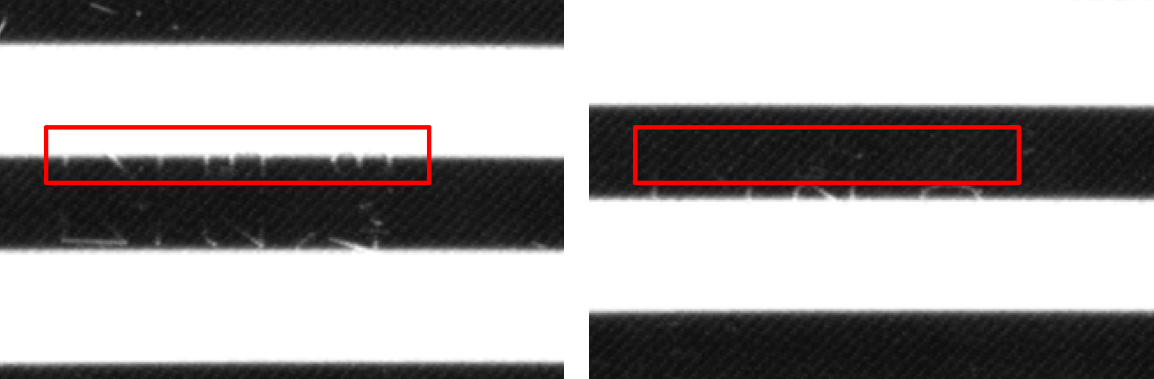
\includegraphics[width=\textwidth]{03_sichtpruefungDurchLichtreflexionen/verfahren/figures/minorScratch}
	\caption[Eingravierung im Glas]{Schlecht erkennbare Eingravierung im Glas, nach Verschiebung des Streifenmusters.}
	\label{img:engraving}
\end{figure}

\noindent
In Abbildung \ref{img:engraving} stellt man fest, dass besonders kleine Defekte der Oberflächenstruktur, wie hier z. B. die Eingravierung, nur zum Teil und auch nur in der Nähe der Übergänge zu erkennen sind.

\p
Daraus lassen sich bestimmte Folgerungen ziehen.
Zunächst decken Streifenmuster nur unmittelbar an den Übergängen zuverlässig Defekte auf.
Das bedeutet, um Defekte an bestimmten Stellen zu erfassen, muss das verwendete Streifenmuster an den Stellen Übergän\-ge haben.
So kann man schließen, dass Muster mit schmaleren Streifen besser geeignet sind, um auch kleinere Oberflächendefekte sichtbar zu machen.
Allerdings führt dies auch dazu, dass stets nur kleine Teile der Defekte zu erkennen sind.
Als Lösung dieses Problems kann man mehrere Streifenmuster verwenden, deren Streifen stets in ihrer Ausbreitungsrichtung verschoben sind.
Verknüpft man die sichtbaren Teile der Defekte, kann man ein vollständiges Gesamtbild erhalten.
In diesem Gesamtbild sollten alle Oberflächendefekte ab einer bestimmten Mindesttiefe sichtbar werden.
Die Mindesttiefe hängt dabei von den Kameraeinstellungen, der Beleuchtungsstärke und den verwendeten Streifenmustern ab.